\section{R Scripts, projects and R Markdown: organizing your work}
\frame{\sectionpage}

\begin{frame}[frame]{R Scripts}
  
  \begin{itemize}
  \item Typing commands in the bottom left Console window is OK, but:
    \begin{itemize}
    \item may need to type commands over again
    \item can use up/down arrows to scroll through previous commands
    \item no easy record of what you did.
    \end{itemize}

  \item File/New/R Script opens new window top left.
  \item enter commands \emph{here}, control-enter or Run button runs
    them (output in console).
  \item select several lines, Run runs all.
  \item \textbf{Have record of what you did}.
  \item Editable: can save list of working commands, with no false
    trails, re-run from start to check analysis reproducible.
  \end{itemize}
  
\end{frame}

\begin{frame}[fragile]{Projects}
  
  \begin{itemize}
  \item Provides a way of putting code and data in one place.
  \item One overarching structure: can have scripts, text windows,
    etc. all open in one place.
  \item When you close a project and re-open it, code and data are as
    you left it.
  \item To create a project, Project-Create Project. Project
    associated with folder (directory). Prompted to create new project
    in new folder, or associate it with existing folder.
  \item Then browse to folder where you want the project, and click
    Create Project.
  \item Can have different projects for eg.\ each assignment, to keep
    them separate.
  \item Helps solve ``folder problem'', because everything in Project folder.
  \end{itemize}
  
\end{frame}

\begin{frame}[fragile]{R Markdown}
  
  \begin{itemize}
  \item Reproducible research: anyone should be able to reproduce
    exactly the analysis you did.
  \item Report and analysis combined (instead of copy-pasting).
  \item Report uses ``markup language'' (simplified HTML) for text
    and formatting.
  \item To add code, insert \emph{code chunk}.
  \item Inside code chunk, put \emph{only} code. This is run when
    document is processed, and output inserted in final document.
  \end{itemize}
  
\end{frame}

\begin{frame}[fragile]{Example R Markdown document}

{\scriptsize  
\begin{verbatim}
This is the title
=================
Here is some data:

```{r}
x=c(10,11,13,14,17,18,22,24,27,41)
x
```

and this is a summary of x:

```{r}
summary(x)
```

Finally, a boxplot of x:

```{r}
boxplot(x)
```

from which we see that x is right-skewed.
\end{verbatim}
  }
  
\end{frame}

\begin{frame}[fragile]{How it looks when ``knitted'', some}
  
  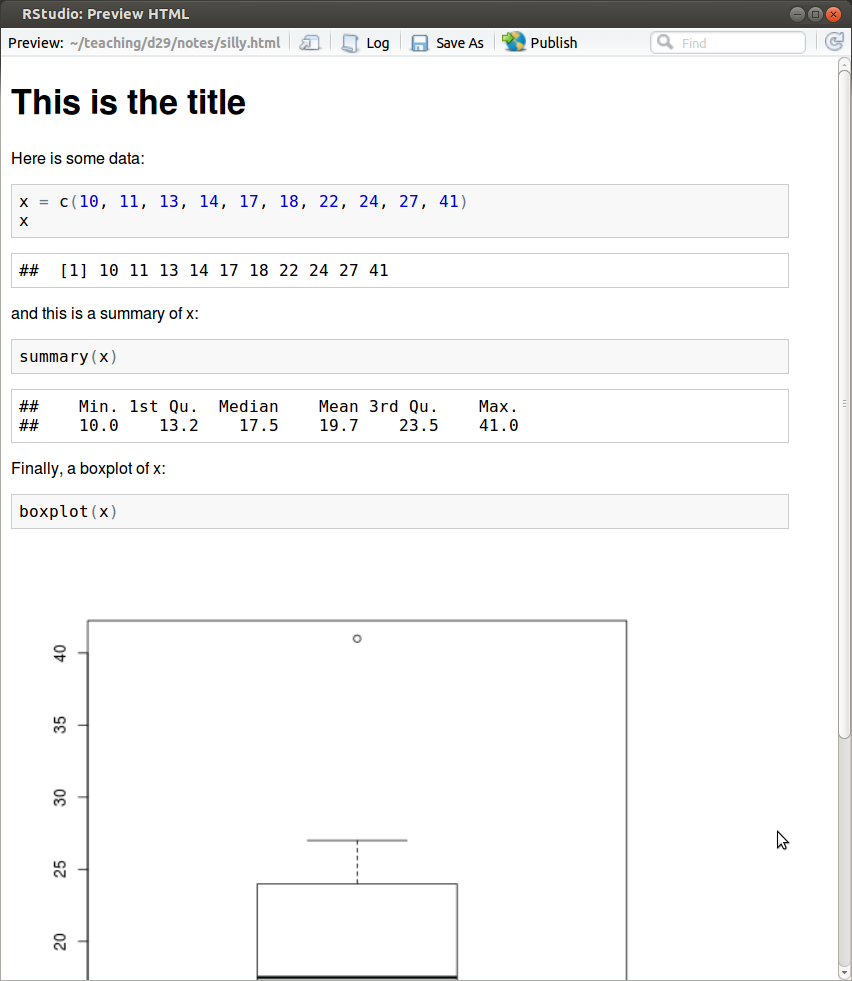
\includegraphics[height=\textheight]{silly}
  
\end{frame}

\begin{frame}[fragile]{Doing it yourself}
  
  \begin{itemize}
  \item See Chapter 19 of The Book.
  \item File-New-R Markdown, pops up new window top left with template.
  \item Save it (just filename, R supplies extension).
  \item Write your report, inserting formatting code.
  \item Insert code chunk by Chunks, Insert Chunk (control-alt-i).
  \item In code chunk, just put the code you want to run. Can produce
    text or graphics output.
  \item To see how it looks, click Knit HTML. Preview window pops up
    showing how results look.
  \item If you don't like it, edit R Markdown and knit again.
  \end{itemize}
  
\end{frame}

\begin{frame}[fragile]{Tidying data}
  
  \begin{itemize}
  \item Most of this from
    \url{http://cran.r-project.org/web/packages/tidyr/vignettes/tidy-data.html}. 
  \item Data don't often come to us in the format that we would like
    them for analysis.
  \item Often, columns should be rows (or vice versa), or columns
    should be combined or split.
  \item Guiding principle (for us): every value belongs to a \emph{variable}
    and an \emph{observation}:
    \begin{itemize}
    \item     A variable contains all values that
    measure the same thing (eg.\ height)
  \item An observation contains all values measured on the same
    subject (eg.\ person.)
  \item Each variable is in a column.
  \item Each observation is in one, or more than one, row.
    \end{itemize}
    
  \end{itemize}
  
\end{frame}

\begin{frame}[fragile]{One variable in multiple columns}
\begin{knitrout}
\definecolor{shadecolor}{rgb}{0.969, 0.969, 0.969}\color{fgcolor}\begin{kframe}
\begin{alltt}
\hlstd{scores}\hlkwb{=}\hlkwd{read.table}\hlstd{(}\hlstr{"scores.txt"}\hlstd{,}\hlkwc{header}\hlstd{=T)}
\hlstd{scores}
\end{alltt}
\begin{verbatim}
##     name assgt.1 test.1 test.2
## 1   Fred      10     45     41
## 2 Angela       9     37     48
## 3  Emily      10     41     45
## 4  David      10     39     33
\end{verbatim}
\end{kframe}
\end{knitrout}

\begin{itemize}
\item \texttt{assgt.1} through \texttt{test.2} are all the same thing
  (scores on an assessment). Combine them into \emph{one} column, with
  a label showing which assessment they belong to. 
   
\end{itemize}
\end{frame}

\begin{frame}[fragile]{\texttt{gather}}
  
  {\small
\begin{knitrout}
\definecolor{shadecolor}{rgb}{0.969, 0.969, 0.969}\color{fgcolor}\begin{kframe}
\begin{alltt}
\hlkwd{library}\hlstd{(tidyr)}
\hlstd{scores2}\hlkwb{=}\hlkwd{gather}\hlstd{(scores,assessment,score,assgt.1}\hlopt{:}\hlstd{test.2) ; scores2}
\end{alltt}
\begin{verbatim}
##      name assessment score
## 1    Fred    assgt.1    10
## 2  Angela    assgt.1     9
## 3   Emily    assgt.1    10
## 4   David    assgt.1    10
## 5    Fred     test.1    45
## 6  Angela     test.1    37
## 7   Emily     test.1    41
## 8   David     test.1    39
## 9    Fred     test.2    41
## 10 Angela     test.2    48
## 11  Emily     test.2    45
## 12  David     test.2    33
\end{verbatim}
\end{kframe}
\end{knitrout}
}

Now can find mean score on each assessment, or make boxplots of scores
for each assessment (side by side). 
\end{frame}

\begin{frame}[fragile]{Anatomy of \texttt{gather}}
  
  Gather requires four things:
  \begin{itemize}
  \item A data frame to work on
  \item What makes the columns different
  \item What makes the columns the same (what the columns to be combined
    are all instances of)
  \item Which columns to ``gather'' together. Can be \texttt{x:y}
    meaning columns \texttt{x} through \texttt{y} inclusive, or a
    vector of column names with \texttt{c()}, or column names to omit
    with \texttt{-}. No quotes needed in column names.
  \end{itemize}
  
\end{frame}

\begin{frame}[fragile]{Splitting things up}
  
Suppose we want to split up that \texttt{assessment} column into two
things': the assessment type \texttt{assess.type} and which number
assessment it is \texttt{assess.num}. That is a job for \texttt{separate}:

{\footnotesize
\begin{knitrout}
\definecolor{shadecolor}{rgb}{0.969, 0.969, 0.969}\color{fgcolor}\begin{kframe}
\begin{alltt}
\hlkwd{separate}\hlstd{(scores2,assessment,}\hlkwc{into}\hlstd{=}\hlkwd{c}\hlstd{(}\hlstr{"assess.type"}\hlstd{,}\hlstr{"assess.num"}\hlstd{),}
         \hlkwc{sep}\hlstd{=}\hlstr{"\textbackslash{}\textbackslash{}."}\hlstd{)}
\end{alltt}
\begin{verbatim}
##      name assess.type assess.num score
## 1    Fred       assgt          1    10
## 2  Angela       assgt          1     9
## 3   Emily       assgt          1    10
## 4   David       assgt          1    10
## 5    Fred        test          1    45
## 6  Angela        test          1    37
## 7   Emily        test          1    41
## 8   David        test          1    39
## 9    Fred        test          2    41
## 10 Angela        test          2    48
## 11  Emily        test          2    45
## 12  David        test          2    33
\end{verbatim}
\end{kframe}
\end{knitrout}
}
  
\end{frame}


\begin{frame}[fragile]{Chaining things together}
  
  To do \texttt{gather} and \texttt{separate} in sequence, there is a
  special notation \texttt{\%>\%} which means
  ``and then''. This lives in package \texttt{dplyr} which we
  investigate later. 


  {\footnotesize
\begin{knitrout}
\definecolor{shadecolor}{rgb}{0.969, 0.969, 0.969}\color{fgcolor}\begin{kframe}
\begin{alltt}
\hlstd{scores} \hlopt
    \hlkwd{gather}\hlstd{(assessment,score,assgt.1}\hlopt{:}\hlstd{test.2)} \hlopt
    \hlkwd{separate}\hlstd{(assessment,}\hlkwc{into}\hlstd{=}\hlkwd{c}\hlstd{(}\hlstr{"assess.type"}\hlstd{,}\hlstr{"assess.num"}\hlstd{),} \hlkwc{sep}\hlstd{=}\hlstr{"\textbackslash{}\textbackslash{}."}\hlstd{)}
\end{alltt}
\begin{verbatim}
##      name assess.type assess.num score
## 1    Fred       assgt          1    10
## 2  Angela       assgt          1     9
## 3   Emily       assgt          1    10
## 4   David       assgt          1    10
## 5    Fred        test          1    45
## 6  Angela        test          1    37
## 7   Emily        test          1    41
## 8   David        test          1    39
## 9    Fred        test          2    41
## 10 Angela        test          2    48
## 11  Emily        test          2    45
## 12  David        test          2    33
\end{verbatim}
\end{kframe}
\end{knitrout}
}
  
\end{frame}


\begin{frame}[fragile]{Anatomy of \texttt{separate}}
  
  This too needs four things:
  
  \begin{itemize}
  \item a data frame
  \item a variable \texttt{x} to separate out into parts
  \item a thing \texttt{into}: a vector of variable names to separate
    \texttt{x} into
  \item a thing \texttt{sep} to specify what to separate on. This is a
    ``regular expression'': the odd-looking code we used means
    ``separate by dot'', but a dot in a regular expression means ``any
    one character'', and we want an actual dot.
  \end{itemize}
  
  
\end{frame}


\begin{frame}[fragile]{More about \texttt{\%>\%}}
    
  When using \texttt{\%>\%}, any function that would have a data frame
  as its first argument has that data frame removed. This applies to
  any such function, thus we can say:
  
\begin{knitrout}
\definecolor{shadecolor}{rgb}{0.969, 0.969, 0.969}\color{fgcolor}\begin{kframe}
\begin{alltt}
\hlstd{scores} \hlopt
   \hlkwd{gather}\hlstd{(assessment,score,assgt.1}\hlopt{:}\hlstd{test.2)} \hlopt
   \hlkwd{head}\hlstd{(}\hlnum{5}\hlstd{)}
\end{alltt}
\begin{verbatim}
##     name assessment score
## 1   Fred    assgt.1    10
## 2 Angela    assgt.1     9
## 3  Emily    assgt.1    10
## 4  David    assgt.1    10
## 5   Fred     test.1    45
\end{verbatim}
\end{kframe}
\end{knitrout}

to show the top 5 lines of the result of \texttt{gather}.
    
  
\end{frame}

\begin{frame}[fragile]{Making separate columns}
  
  Consider this:
  
\begin{knitrout}
\definecolor{shadecolor}{rgb}{0.969, 0.969, 0.969}\color{fgcolor}\begin{kframe}
\begin{alltt}
\hlstd{weather}\hlkwb{=}\hlkwd{read.table}\hlstd{(}\hlstr{"weather.txt"}\hlstd{,}\hlkwc{header}\hlstd{=T)}
\hlstd{weather}
\end{alltt}
\begin{verbatim}
##          date type temperature
## 1  2010-12-01 tmax        29.9
## 2  2010-12-01 tmin        13.8
## 3  2010-02-02 tmax        27.3
## 4  2010-02-02 tmin        14.4
## 5  2010-11-02 tmax        31.3
## 6  2010-11-02 tmin        16.3
## 7  2010-02-03 tmax        24.1
## 8  2010-02-03 tmin        14.4
## 9  2010-07-03 tmax        28.6
## 10 2010-07-03 tmin        17.5
\end{verbatim}
\end{kframe}
\end{knitrout}

  
\end{frame}

\begin{frame}[fragile]{\texttt{spread}}

\texttt{temperature} is certainly temperature, but \texttt{type}
is two kinds of temperature: daily maximum and 
daily minimum. Two separate variables, and thus need to be
in two separate columns. Inverse of \texttt{gather}:

\begin{knitrout}
\definecolor{shadecolor}{rgb}{0.969, 0.969, 0.969}\color{fgcolor}\begin{kframe}
\begin{alltt}
\hlstd{weather} \hlopt \hlkwd{spread}\hlstd{(type,temperature)}
\end{alltt}
\begin{verbatim}
##         date tmax tmin
## 1 2010-02-02 27.3 14.4
## 2 2010-02-03 24.1 14.4
## 3 2010-07-03 28.6 17.5
## 4 2010-11-02 31.3 16.3
## 5 2010-12-01 29.9 13.8
\end{verbatim}
\end{kframe}
\end{knitrout}

\texttt{spread} needs two things: the variable for dividing into
groups (used as names for new variables), and the variable to be
divided. If not used in a \texttt{\%>\%} sequence, needs data frame on
front. 

\end{frame}

\begin{frame}[fragile]{\texttt{dplyr}: doing things to tidy data frames}
  
  Real-life data frames, even after tidying, don't always  contain
  what we want. \texttt{dplyr} helps to ``bash things into shape'':
  
  \begin{itemize}
  \item Selecting rows (observations) (\texttt{filter})
  \item Sorting rows by variables (\texttt{arrange})
  \item Selecting columns (variables) (\texttt{select})
  \item Creating new variables (\texttt{mutate})
  \item Summarizing variables (\texttt{summarise})
  \item Randomly sampling rows (\texttt{sample\_n} and \texttt{sample\_frac})
  \end{itemize}
  
  This based on \url{http://cran.rstudio.com/web/packages/dplyr/vignettes/introduction.html}.

  Start with:
\begin{knitrout}
\definecolor{shadecolor}{rgb}{0.969, 0.969, 0.969}\color{fgcolor}\begin{kframe}
\begin{alltt}
\hlkwd{library}\hlstd{(dplyr)}
\end{alltt}
\end{kframe}
\end{knitrout}

\end{frame}


\begin{frame}[fragile]{Selecting rows (1)}
  
  Start with somewhat-tidy marks data frame:
  
\begin{knitrout}
\definecolor{shadecolor}{rgb}{0.969, 0.969, 0.969}\color{fgcolor}\begin{kframe}
\begin{alltt}
\hlstd{scores2}
\end{alltt}
\begin{verbatim}
##      name assessment score
## 1    Fred    assgt.1    10
## 2  Angela    assgt.1     9
## 3   Emily    assgt.1    10
## 4   David    assgt.1    10
## 5    Fred     test.1    45
## 6  Angela     test.1    37
## 7   Emily     test.1    41
## 8   David     test.1    39
## 9    Fred     test.2    41
## 10 Angela     test.2    48
## 11  Emily     test.2    45
## 12  David     test.2    33
\end{verbatim}
\end{kframe}
\end{knitrout}


  
  
\end{frame}

\begin{frame}[fragile]{Selecting rows (2)}
  
  To select just Angela's marks (note \texttt{==}):
  
\begin{knitrout}
\definecolor{shadecolor}{rgb}{0.969, 0.969, 0.969}\color{fgcolor}\begin{kframe}
\begin{alltt}
\hlkwd{filter}\hlstd{(scores2,name}\hlopt{==}\hlstr{"Angela"}\hlstd{)}
\end{alltt}
\begin{verbatim}
##     name assessment score
## 1 Angela    assgt.1     9
## 2 Angela     test.1    37
## 3 Angela     test.2    48
\end{verbatim}
\end{kframe}
\end{knitrout}

or just Angela's test 1 mark (``and'' implied):

\begin{knitrout}
\definecolor{shadecolor}{rgb}{0.969, 0.969, 0.969}\color{fgcolor}\begin{kframe}
\begin{alltt}
\hlkwd{filter}\hlstd{(scores2,name}\hlopt{==}\hlstr{"Angela"}\hlstd{,assessment}\hlopt{==}\hlstr{"test.1"}\hlstd{)}
\end{alltt}
\begin{verbatim}
##     name assessment score
## 1 Angela     test.1    37
\end{verbatim}
\end{kframe}
\end{knitrout}
  
\end{frame}

\begin{frame}[fragile]{Selecting rows (3)}
  
Select marks which belong either to assignment 1 or to test 1:

\begin{knitrout}
\definecolor{shadecolor}{rgb}{0.969, 0.969, 0.969}\color{fgcolor}\begin{kframe}
\begin{alltt}
\hlkwd{filter}\hlstd{(scores2,}
    \hlstd{assessment}\hlopt{==}\hlstr{"assgt.1"} \hlopt{|} \hlstd{assessment}\hlopt{==}\hlstr{"test.1"}\hlstd{)}
\end{alltt}
\begin{verbatim}
##     name assessment score
## 1   Fred    assgt.1    10
## 2 Angela    assgt.1     9
## 3  Emily    assgt.1    10
## 4  David    assgt.1    10
## 5   Fred     test.1    45
## 6 Angela     test.1    37
## 7  Emily     test.1    41
## 8  David     test.1    39
\end{verbatim}
\end{kframe}
\end{knitrout}
  
\end{frame}

\begin{frame}[fragile]{Selecting rows (4)}
  
Select the marks that are over 40:

\begin{knitrout}
\definecolor{shadecolor}{rgb}{0.969, 0.969, 0.969}\color{fgcolor}\begin{kframe}
\begin{alltt}
\hlkwd{filter}\hlstd{(scores2,score}\hlopt{>}\hlnum{40}\hlstd{)}
\end{alltt}
\begin{verbatim}
##     name assessment score
## 1   Fred     test.1    45
## 2  Emily     test.1    41
## 3   Fred     test.2    41
## 4 Angela     test.2    48
## 5  Emily     test.2    45
\end{verbatim}
\end{kframe}
\end{knitrout}
  
\end{frame}

\begin{frame}[fragile]{Ordering rows (1)}
  
To sort rows into order (by one or more variables), use \texttt{arrange}:

{\small
\begin{knitrout}
\definecolor{shadecolor}{rgb}{0.969, 0.969, 0.969}\color{fgcolor}\begin{kframe}
\begin{alltt}
\hlkwd{arrange}\hlstd{(scores2,name)}
\end{alltt}
\begin{verbatim}
##      name assessment score
## 1  Angela    assgt.1     9
## 2  Angela     test.1    37
## 3  Angela     test.2    48
## 4   David    assgt.1    10
## 5   David     test.1    39
## 6   David     test.2    33
## 7   Emily    assgt.1    10
## 8   Emily     test.1    41
## 9   Emily     test.2    45
## 10   Fred    assgt.1    10
## 11   Fred     test.1    45
## 12   Fred     test.2    41
\end{verbatim}
\end{kframe}
\end{knitrout}
}
  
\end{frame}

\begin{frame}[fragile]{Ordering rows (2)}
  
In descending order:

{\small
\begin{knitrout}
\definecolor{shadecolor}{rgb}{0.969, 0.969, 0.969}\color{fgcolor}\begin{kframe}
\begin{alltt}
\hlkwd{arrange}\hlstd{(scores2,}\hlkwd{desc}\hlstd{(score))}
\end{alltt}
\begin{verbatim}
##      name assessment score
## 1  Angela     test.2    48
## 2    Fred     test.1    45
## 3   Emily     test.2    45
## 4   Emily     test.1    41
## 5    Fred     test.2    41
## 6   David     test.1    39
## 7  Angela     test.1    37
## 8   David     test.2    33
## 9    Fred    assgt.1    10
## 10  Emily    assgt.1    10
## 11  David    assgt.1    10
## 12 Angela    assgt.1     9
\end{verbatim}
\end{kframe}
\end{knitrout}
}
  
\end{frame}


\begin{frame}[fragile]{Ordering rows (3)}
  
By name, breaking ties in descending order of score:

{\small
\begin{knitrout}
\definecolor{shadecolor}{rgb}{0.969, 0.969, 0.969}\color{fgcolor}\begin{kframe}
\begin{alltt}
\hlkwd{arrange}\hlstd{(scores2,name,}\hlkwd{desc}\hlstd{(score))}
\end{alltt}
\begin{verbatim}
##      name assessment score
## 1  Angela     test.2    48
## 2  Angela     test.1    37
## 3  Angela    assgt.1     9
## 4   David     test.1    39
## 5   David     test.2    33
## 6   David    assgt.1    10
## 7   Emily     test.2    45
## 8   Emily     test.1    41
## 9   Emily    assgt.1    10
## 10   Fred     test.1    45
## 11   Fred     test.2    41
## 12   Fred    assgt.1    10
\end{verbatim}
\end{kframe}
\end{knitrout}
}
  
\end{frame}

\begin{frame}[fragile]{Selecting columns (variables) (1)}

  \texttt{select} selects columns. You choose columns the same way as
  in \texttt{gather}.
  For
  example, to pull out just the marks:
  
\begin{knitrout}
\definecolor{shadecolor}{rgb}{0.969, 0.969, 0.969}\color{fgcolor}\begin{kframe}
\begin{alltt}
\hlkwd{select}\hlstd{(scores2,score)}
\end{alltt}
\begin{verbatim}
##    score
## 1     10
## 2      9
## 3     10
## 4     10
## 5     45
## 6     37
## 7     41
## 8     39
## 9     41
## 10    48
## 11    45
## 12    33
\end{verbatim}
\end{kframe}
\end{knitrout}
  
\end{frame}

\begin{frame}[fragile]{Selcting columns (variables) (2)}
  
  And to pull out everything but the names:
  
\begin{knitrout}
\definecolor{shadecolor}{rgb}{0.969, 0.969, 0.969}\color{fgcolor}\begin{kframe}
\begin{alltt}
\hlkwd{select}\hlstd{(scores2,}\hlopt{-}\hlstd{name)}
\end{alltt}
\begin{verbatim}
##    assessment score
## 1     assgt.1    10
## 2     assgt.1     9
## 3     assgt.1    10
## 4     assgt.1    10
## 5      test.1    45
## 6      test.1    37
## 7      test.1    41
## 8      test.1    39
## 9      test.2    41
## 10     test.2    48
## 11     test.2    45
## 12     test.2    33
\end{verbatim}
\end{kframe}
\end{knitrout}
  
\end{frame}

\begin{frame}[fragile]{Selcting columns (variables) (3)}
  
Or, select ``assessment through score'':
  
\begin{knitrout}
\definecolor{shadecolor}{rgb}{0.969, 0.969, 0.969}\color{fgcolor}\begin{kframe}
\begin{alltt}
\hlkwd{select}\hlstd{(scores2,assessment}\hlopt{:}\hlstd{score)}
\end{alltt}
\begin{verbatim}
##    assessment score
## 1     assgt.1    10
## 2     assgt.1     9
## 3     assgt.1    10
## 4     assgt.1    10
## 5      test.1    45
## 6      test.1    37
## 7      test.1    41
## 8      test.1    39
## 9      test.2    41
## 10     test.2    48
## 11     test.2    45
## 12     test.2    33
\end{verbatim}
\end{kframe}
\end{knitrout}
  
\end{frame}

\begin{frame}[fragile]{Chaining things together}
  
Any of the \texttt{dplyr} functions, like the \texttt{tidyr}
functions, can be chained together in sequence. Again, remove the
first data frame argument to any of the functions. Thus, to select
everything but name and display the first 5 rows:

\begin{knitrout}
\definecolor{shadecolor}{rgb}{0.969, 0.969, 0.969}\color{fgcolor}\begin{kframe}
\begin{alltt}
\hlstd{scores2} \hlopt \hlkwd{select}\hlstd{(}\hlopt{-}\hlstd{name)} \hlopt \hlkwd{head}\hlstd{(}\hlnum{5}\hlstd{)}
\end{alltt}
\begin{verbatim}
##   assessment score
## 1    assgt.1    10
## 2    assgt.1     9
## 3    assgt.1    10
## 4    assgt.1    10
## 5     test.1    45
\end{verbatim}
\end{kframe}
\end{knitrout}
  
\end{frame}

\begin{frame}[fragile]{Finding the different ones: \texttt{distinct}}
  
  ``What are the different
  assessments?'' Easiest done in a chain:
  
\begin{knitrout}
\definecolor{shadecolor}{rgb}{0.969, 0.969, 0.969}\color{fgcolor}\begin{kframe}
\begin{alltt}
\hlstd{scores2} \hlopt \hlkwd{select}\hlstd{(assessment)} \hlopt \hlkwd{distinct}\hlstd{()}
\end{alltt}
\begin{verbatim}
##   assessment
## 1    assgt.1
## 2     test.1
## 3     test.2
\end{verbatim}
\end{kframe}
\end{knitrout}
  
\end{frame}

\begin{frame}[fragile]{What does this one do?}
  
\begin{knitrout}
\definecolor{shadecolor}{rgb}{0.969, 0.969, 0.969}\color{fgcolor}\begin{kframe}
\begin{alltt}
\hlstd{scores2} \hlopt \hlkwd{select}\hlstd{(}\hlopt{-}\hlstd{name)} \hlopt \hlkwd{head}\hlstd{(}\hlnum{5}\hlstd{)} \hlopt \hlkwd{distinct}\hlstd{()}
\end{alltt}
\begin{verbatim}
##   assessment score
## 1    assgt.1    10
## 2    assgt.1     9
## 3     test.1    45
\end{verbatim}
\end{kframe}
\end{knitrout}
  
This shows the distinct assessment-score patterns (several people had
the same score on the same assessment, so even though we looked at the
top 5 lines of the result, several of them were identical, so we only
got 3 distinct ones).
  
\end{frame}


\begin{frame}[fragile]{Creating new columns using \texttt{mutate}}
  
  Suppose the assignment is out of 10, the tests are out of 50, and we
  want to create a new column that is percentages:
  
  {\small
\begin{knitrout}
\definecolor{shadecolor}{rgb}{0.969, 0.969, 0.969}\color{fgcolor}\begin{kframe}
\begin{alltt}
\hlkwd{mutate}\hlstd{(scores2,}\hlkwc{out.of}\hlstd{=}\hlkwd{c}\hlstd{(}\hlkwd{rep}\hlstd{(}\hlnum{10}\hlstd{,}\hlnum{4}\hlstd{),}\hlkwd{rep}\hlstd{(}\hlnum{50}\hlstd{,}\hlnum{8}\hlstd{)),}
               \hlkwc{percent}\hlstd{=score}\hlopt{/}\hlstd{out.of}\hlopt{*}\hlnum{100}\hlstd{)}
\end{alltt}
\begin{verbatim}
##      name assessment score out.of percent
## 1    Fred    assgt.1    10     10     100
## 2  Angela    assgt.1     9     10      90
## 3   Emily    assgt.1    10     10     100
## 4   David    assgt.1    10     10     100
## 5    Fred     test.1    45     50      90
## 6  Angela     test.1    37     50      74
## 7   Emily     test.1    41     50      82
## 8   David     test.1    39     50      78
## 9    Fred     test.2    41     50      82
## 10 Angela     test.2    48     50      96
## 11  Emily     test.2    45     50      90
## 12  David     test.2    33     50      66
\end{verbatim}
\end{kframe}
\end{knitrout}
}
  
\end{frame}

\begin{frame}[fragile]{Summarizing values}
  
  Use \texttt{summarise} or \texttt{summarize}:
  
\begin{knitrout}
\definecolor{shadecolor}{rgb}{0.969, 0.969, 0.969}\color{fgcolor}\begin{kframe}
\begin{alltt}
\hlkwd{summarise}\hlstd{(scores2,}\hlkwc{mean.score}\hlstd{=}\hlkwd{mean}\hlstd{(score))}
\end{alltt}
\begin{verbatim}
##   mean.score
## 1   30.66667
\end{verbatim}
\end{kframe}
\end{knitrout}

Not useful yet, but very useful in making summaries by group (later).
  
\end{frame}

\begin{frame}[fragile]{Random samples of rows}
  


By the number of rows you want:

\begin{knitrout}
\definecolor{shadecolor}{rgb}{0.969, 0.969, 0.969}\color{fgcolor}\begin{kframe}
\begin{alltt}
\hlkwd{sample_n}\hlstd{(scores2,}\hlnum{5}\hlstd{)}
\end{alltt}
\begin{verbatim}
##      name assessment score
## 12  David     test.2    33
## 2  Angela    assgt.1     9
## 3   Emily    assgt.1    10
## 6  Angela     test.1    37
## 4   David    assgt.1    10
\end{verbatim}
\end{kframe}
\end{knitrout}

or the fraction of rows you want:

\begin{knitrout}
\definecolor{shadecolor}{rgb}{0.969, 0.969, 0.969}\color{fgcolor}\begin{kframe}
\begin{alltt}
\hlkwd{sample_frac}\hlstd{(scores2,}\hlnum{0.25}\hlstd{)}
\end{alltt}
\begin{verbatim}
##      name assessment score
## 10 Angela     test.2    48
## 3   Emily    assgt.1    10
## 11  Emily     test.2    45
\end{verbatim}
\end{kframe}
\end{knitrout}
  
\end{frame}


\begin{frame}[fragile]{Doing things by groups}
  
  Start with \texttt{group\_by}. Then use \texttt{summarise()} or
  whatever as needed. This seems to work most naturally in a chain.
  
  To find the mean score on each assessment:
  
\begin{knitrout}
\definecolor{shadecolor}{rgb}{0.969, 0.969, 0.969}\color{fgcolor}\begin{kframe}
\begin{alltt}
\hlstd{scores2} \hlopt \hlkwd{group_by}\hlstd{(assessment)} \hlopt
   \hlkwd{summarise}\hlstd{(} \hlkwc{assess.mean}\hlstd{=}\hlkwd{mean}\hlstd{(score),}
              \hlkwc{assess.sd}\hlstd{=}\hlkwd{sd}\hlstd{(score)}
            \hlstd{)}
\end{alltt}
\begin{verbatim}
## Source: local data frame [3 x 3]
## 
##   assessment assess.mean assess.sd
##       (fctr)       (dbl)     (dbl)
## 1    assgt.1        9.75   0.50000
## 2     test.1       40.50   3.41565
## 3     test.2       41.75   6.50000
\end{verbatim}
\end{kframe}
\end{knitrout}
  
\end{frame}

\begin{frame}[fragile]{How many assessments did each person do?}
  
\begin{knitrout}
\definecolor{shadecolor}{rgb}{0.969, 0.969, 0.969}\color{fgcolor}\begin{kframe}
\begin{alltt}
\hlstd{scores2} \hlopt \hlkwd{group_by}\hlstd{(name)} \hlopt
   \hlkwd{summarize}\hlstd{(}\hlkwc{how.many}\hlstd{=}\hlkwd{n}\hlstd{())}
\end{alltt}
\begin{verbatim}
## Source: local data frame [4 x 2]
## 
##     name how.many
##   (fctr)    (int)
## 1 Angela        3
## 2  David        3
## 3  Emily        3
## 4   Fred        3
\end{verbatim}
\end{kframe}
\end{knitrout}
  

This is actually ``how many times did each name appear in the original
data frame?''.
\end{frame}
